\documentclass{beamer}

\mode<presentation>
{
  \usetheme{Warsaw}
  \usecolortheme{default}
  \usefonttheme{default}
  \setbeamertemplate{navigation symbols}{}
  \setbeamertemplate{caption}[numbered]
} 

\usepackage[english]{babel}
\usepackage[utf8x]{inputenc}


\title{Eet jij ongezond?}
\author{Mitchell Scheidsbach}
\institute{Hogeschool Rotterdam}
\date{\today}

\begin{document}

\begin{frame}
  \titlepage
\end{frame}


\begin{frame}{Er zijn 9 mensen geïnterviewd\newline Het 4e interview geloof je nooit}

\begin{table}
	\centering
	\begin{tabular}{l|r}
		Voedsel & Aantal \\\hline
		Fruit & 4 \\
		Groente & 5 \\
		Fast food & 7 \\
		Chips & 4 \\
		Koolhydraten \\ 6
	\end{tabular}
\end{table}

\end{frame}


\begin{frame}{Er zijn verkopen geobserveerd\newline De resultaten zijn ongelofelijk}

\begin{figure}[!ht]
	\centering
	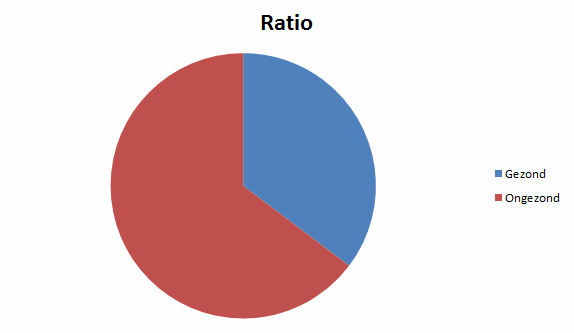
\includegraphics[width=0.8\textwidth]{piechart.png}
	\centering
	\label{label:file_name}
\end{figure}

\end{frame}


\begin{frame}{Deze enquête is helemaal in!\newline De 2e vraag is hilarisch.}
Helaas zijn de resultaten nog niet verwerkt

\begin{figure}[!ht]
	\centering
	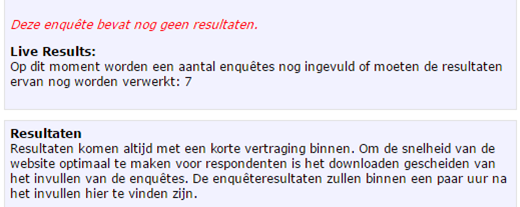
\includegraphics[width=0.7\textwidth]{resultaten.png}
	\centering
	\label{label:file_name}
\end{figure}
\end{frame}


\begin{frame}{Het resultaat van het onderzoek is binnen\newline We konden onze ogen niet geloven}
\
\centering\LARGE Er wordt vooral ongezond gegeten!
\end{frame}

\end{document}
